\documentclass[5p,times]{elsarticle}

\usepackage{amsmath,amssymb,amsfonts}
\usepackage{graphicx}
\usepackage{booktabs}
\usepackage{multirow}
\usepackage{xcolor}
\usepackage{textcomp}
\usepackage{tikz}
\usepackage{pgfplots}
\usepackage{algorithm}
\usepackage{algpseudocode}
\usepackage{url}
\usepackage{hyperref}

\usetikzlibrary{shapes.geometric, arrows.meta, positioning, fit, backgrounds, calc}
\pgfplotsset{compat=1.16}

\hypersetup{colorlinks=true, linkcolor=blue, citecolor=blue, urlcolor=blue}

\emergencystretch=1.5em

\definecolor{xsdnblue}{RGB}{31,90,166}
\definecolor{xsdnteal}{RGB}{0,140,140}
\definecolor{xsdnorange}{RGB}{217,119,32}
\definecolor{xsdnred}{RGB}{190,45,45}
\definecolor{xsdngray}{RGB}{110,110,110}
\definecolor{xsdngreen}{RGB}{55,130,60}
\definecolor{cmlow}{RGB}{235,242,250}
\definecolor{cmhigh}{RGB}{31,90,166}

\journal{Computers \& Security}

\begin{document}

\begin{frontmatter}

\title{XAI-SDN: An explainable entropy-guided machine learning framework for real-time DDoS detection in software defined networks}

\author[a]{Adeel Ahmad}
\author[a]{Ali Akarma}
\author[b]{Hasan Razzaqi\corref{cor1}}
\ead{hasan.razzaqi@aou.org.bh}
\author[a]{Toqeer Ali Syed}
\author[c]{Hammad Muneer}
\author[b]{Salman Jan}

\affiliation[a]{organization={Faculty of Computer and Information Systems, Islamic University of Madinah}, city={Madinah}, country={Saudi Arabia}}
\affiliation[b]{organization={Faculty of Computer Studies, Arab Open University}, country={Bahrain}}
\affiliation[c]{organization={Department of Computer Science, Islamia University of Bahawalpur}, city={Bahawalpur}, country={Pakistan}}

\cortext[cor1]{Corresponding author.}

\begin{abstract}
Software Defined Networking (SDN) centralizes network control in a programmable controller, and this very centralization exposes a single point of failure: a successful Distributed Denial of Service (DDoS) attack against the controller or its control channel can render the entire network inoperable. Machine learning (ML) detectors achieve high accuracy on this task but typically operate as black boxes, which prevents security operators from validating and auditing individual detection decisions. This paper presents XAI-SDN, a lightweight, interpretable framework for real-time DDoS detection in SDN environments. XAI-SDN augments the 80 statistical flow features produced by CICFlowMeter with eight Shannon entropy metrics maintained by a constant-time $\mathcal{O}(1)$ rolling-window algorithm, classifies the resulting 88-dimensional flow representation with a Random Forest, and attaches a per-prediction SHAP TreeExplainer attribution to every raised alert. On a fixed temporal split of the complete CIC-DDoS2019 SYN partition (3.59 million flows, no subsampling), XAI-SDN attains 99.9987\% accuracy, 99.9621\% macro F1, and an AUC-ROC of 1.0000, with only 14 misclassifications among 1,077,798 held-out flows. The pipeline sustains 0.0165 ms per flow (60,606 flows/s) without explanation generation and 0.5122 ms per flow (1,953 flows/s) with full SHAP support under the benchmark's 99.14\% DDoS prevalence. A multi-seed ablation with Wilcoxon signed-rank testing shows that the entropy and CICFlowMeter feature families are complementary, and an explicit robustness analysis quantifies how split methodology affects the achievable false positive rate, positioning XAI-SDN as a step toward balancing detection performance and operational transparency in next-generation SDN security.
\end{abstract}

\begin{keyword}
DDoS detection \sep software defined networks \sep explainable AI \sep Shannon entropy \sep random forest \sep SHAP \sep network security
\end{keyword}

\end{frontmatter}

\section{Introduction}
\label{sec:intro}

Software Defined Networking (SDN) has transformed the management of network infrastructure by decoupling the data plane from the control plane, enabling centralized, programmatic governance of the network through a dedicated controller~\cite{mckeown2008openflow,kreutz2015sdn}. The paradigm is widely deployed in enterprise data centres and cloud infrastructure because it offers flexibility, global network visibility, and dynamic traffic engineering. Centralization, however, has a structural cost: the controller constitutes a single point of failure, and a successful Distributed Denial of Service (DDoS) attack that saturates the controller or its control channel can render the entire network inoperable.

Modern DDoS campaigns combine volumetric flooding---UDP amplification, TCP SYN floods, and ICMP sweeps---with application-layer vectors such as HTTP floods and SlowLoris~\cite{sharafaldin2019ddos,akarma2026agents}. Machine learning (ML) has become the leading detection approach for SDN because learned classifiers generalize beyond the fixed patterns of signature-based systems. Yet the models deployed in practice are predominantly black boxes: they do not explain why a given flow was classified as malicious. In security operations this opacity is a concrete liability, because operators must validate, audit, and act on each detection decision, and emerging regulatory frameworks increasingly require that automated security decisions be traceable~\cite{toqeer2026climate,jan2025blockchain,arrieta2020xai}.

Three requirements must therefore be satisfied simultaneously by a practical SDN DDoS detector: (\emph{i}) detection quality high enough to protect an infrastructure in which a single missed volumetric attack is catastrophic; (\emph{ii}) per-flow processing cost low enough to keep pace with controller-scale flow arrival rates; and (\emph{iii}) per-decision transparency sufficient for operator triage and audit. Existing work typically addresses at most two of the three: entropy-based statistical detectors are fast and interpretable but less accurate than learned models~\cite{mousavi2015early}, deep detectors are accurate but opaque and computationally heavy, and post-hoc explanation of deep models is usually too slow for per-flow operation.

This paper presents XAI-SDN, a framework designed around all three requirements at once. XAI-SDN enriches the standard CICFlowMeter statistical feature set with eight Shannon entropy metrics maintained by a constant-time rolling algorithm, classifies flows with a Random Forest, and generates an exact SHAP TreeExplainer attribution for every alert it raises. The design deliberately pairs an ensemble model whose accuracy is competitive with deep alternatives with an explanation method that is exact and fast for tree ensembles, so that transparency is obtained without sacrificing throughput.

The main contributions are as follows.
\begin{itemize}
\item \textbf{Entropy-guided feature augmentation.} An original feature augmentation approach that enriches the 80 CICFlowMeter flow features with eight interpretable Shannon entropy metrics computed over a sliding window, supported by an $\mathcal{O}(1)$ rolling update algorithm (Section~\ref{sec:math}) whose per-flow cost is independent of the window size.
\item \textbf{Explainability-integrated detection pipeline.} A per-prediction pipeline coupling a Random Forest classifier with SHAP TreeExplainer so that every dispatched alert carries an exact feature attribution, enabling operator triage directly from the alert payload (Section~\ref{sec:framework}).
\item \textbf{Full-scale empirical evaluation.} A comprehensive evaluation on the entire SYN partition of CIC-DDoS2019---3.59 million flows without subsampling---under a leakage-free temporal split, complemented by a multi-seed ablation study with Wilcoxon signed-rank significance testing (Sections~\ref{sec:setup}--\ref{sec:comparative}).
\item \textbf{Honest operational characterization.} A corrected latency analysis that accounts for SHAP invocation under realistic DDoS prevalence, and an explicit false-positive-rate robustness analysis showing how split methodology changes the attainable operating point (Section~\ref{sec:results}), both of which are routinely omitted in prior work.
\end{itemize}

The remainder of the paper is organized as follows. Section~\ref{sec:related} reviews related work. Section~\ref{sec:threat} defines the threat model and formalizes the detection problem. Section~\ref{sec:framework} describes the XAI-SDN architecture and Section~\ref{sec:math} its mathematical foundation. Section~\ref{sec:setup} details the experimental setup. Section~\ref{sec:results} reports detection, latency, and explainability results. Section~\ref{sec:comparative} presents the ablation and baseline comparison. Section~\ref{sec:discussion} discusses deployment considerations and limitations, and Section~\ref{sec:conclusion} concludes.

\section{Related work}
\label{sec:related}

\subsection{Entropy-based DDoS detection in SDN}
Entropy is a natural measure of the distributional concentration that characterizes flooding behaviour~\cite{nychis2008entropy}. Mousavi and St-Hilaire~\cite{mousavi2015early} showed that entropy-based early detection at the SDN controller substantially reduces attack damage, using a simple threshold on destination-address entropy. Lall et al.~\cite{lall2006entropy} established that entropy estimation over sliding windows of data streams is an efficient primitive for anomaly detection at line rate. These approaches are computationally attractive and directly interpretable, but a fixed entropy threshold cannot capture the interaction between distributional and per-flow statistical evidence, which limits detection quality relative to learned models. XAI-SDN continues this tradition but repositions entropy: rather than acting as the detector itself, $\mathcal{O}(1)$ rolling entropy becomes an early-stage feature generator, so that discriminative distributional statistics are available both to the classifier and to the SHAP explainer.

\subsection{Machine learning for SDN DDoS detection}
ML-based SDN DDoS detection has been studied extensively, with ensemble methods receiving particular attention for their accuracy, efficiency, and native feature-ranking capability. The CIC-IDS and CIC-DDoS benchmark families~\cite{sharafaldin2018cicids,sharafaldin2019ddos} standardized flow-level evaluation through the CICFlowMeter feature extractor and made large-scale comparison possible. Across this literature, tree ensembles such as Random Forest~\cite{breiman2001rf} and gradient boosting consistently rank among the strongest performers at a small fraction of the inference cost of deep models, a pattern our baseline study (Section~\ref{sec:comparative}) reproduces. However, published evaluations frequently rely on random splits of temporally ordered captures, which leaks near-duplicate flows across the split boundary and overstates operational performance; Section~\ref{sec:results} quantifies this effect explicitly.

\subsection{Explainable AI for intrusion detection}
Explainable AI (XAI) offers post-hoc and intrinsic interpretability mechanisms for security models~\cite{arrieta2020xai}. Lundberg and Lee~\cite{lundberg2017shap} introduced SHAP, which unifies several existing explanation approaches under a single additive-attribution framework with consistency guarantees, and TreeSHAP~\cite{lundberg2020treeshap} extends it to tree-based models with exact polynomial-time computation. Gaspar et al.~\cite{gaspar2024xai} applied LIME and SHAP to a multi-layer-perceptron intrusion detector, demonstrating the operational value of attributions but paying the latency cost of model-agnostic explanation over a deep model. Table~\ref{tab:relwork} situates XAI-SDN in this landscape. To the best of our knowledge, the combination of $\mathcal{O}(1)$ entropy augmentation, Random Forest classification, and exact per-prediction TreeSHAP explanation, evaluated with a realistic characterization of explanation latency under actual DDoS prevalence, has not previously been demonstrated.

\begin{table*}[!t]
\centering
\caption{Qualitative comparison of XAI-SDN with representative prior approaches.}
\label{tab:relwork}
\small
\setlength{\tabcolsep}{4.5pt}
\resizebox{\textwidth}{!}{%
\begin{tabular}{@{}llllll@{}}
\toprule
\textbf{Approach} & \textbf{Detection mechanism} & \textbf{Entropy features} & \textbf{Per-flow XAI} & \textbf{Explanation cost} & \textbf{SDN integration} \\
\midrule
Mousavi and St-Hilaire~\cite{mousavi2015early} & Entropy threshold & Destination IP only & Intrinsic & Negligible & Controller-embedded \\
Lall et al.~\cite{lall2006entropy} & Streaming entropy estim. & Stream sketches & Intrinsic & Negligible & Not addressed \\
Nychis et al.~\cite{nychis2008entropy} & Entropy anomaly corr. & Multiple distributions & Intrinsic & Negligible & Not addressed \\
Gaspar et al.~\cite{gaspar2024xai} & MLP classifier & None & Post-hoc LIME/SHAP & High (model-agnostic) & Not addressed \\
\textbf{XAI-SDN (this work)} & \textbf{RF on 88-dim features} & \textbf{Eight $\mathcal{O}(1)$ rolling} & \textbf{Exact TreeSHAP} & \textbf{0.5 ms per alert} & \textbf{Controller-embedded} \\
\bottomrule
\end{tabular}%
}
\end{table*}

\section{Threat model and problem formulation}
\label{sec:threat}

\subsection{Threat model}
We consider a volumetric DDoS adversary targeting an SDN deployment. The adversary controls a botnet of compromised hosts and launches TCP SYN flood traffic toward victims reachable through the SDN data plane, with the second-order objective of exhausting the controller through the table-miss path: each unmatched flow triggers a \texttt{packet\_in} event, so a sufficiently high rate of spoofed flows saturates the control channel and controller CPU. The adversary may spoof source addresses and vary packet timing but does not control the SDN controller, the switches' management interfaces, or the detection module itself; adaptive adversaries that shape traffic specifically to evade entropy features are out of scope and discussed as future work in Section~\ref{sec:discussion}. The defender observes flow statistics exported by OpenFlow switches and must decide, per flow and in real time, whether the flow belongs to an attack, and must justify that decision to a human operator.

\subsection{Problem formulation}
Let $f_i$ denote the $i$-th flow observed at the controller and let $\mathbf{x}_i \in \mathbb{R}^{d}$ with $d=88$ be its feature representation, composed of $80$ CICFlowMeter statistical features and $8$ windowed entropy features (Section~\ref{sec:math}). The detection task is to learn a scoring function $g_{\theta}\colon \mathbb{R}^{d} \to [0,1]$ and threshold $\tau$ such that the decision rule
\begin{equation}
\hat{y}_i = \mathbb{1}\bigl[g_{\theta}(\mathbf{x}_i) \geq \tau\bigr]
\label{eq:decision}
\end{equation}
maximizes macro-averaged F1 under severe class imbalance, subject to a per-flow latency budget $L$ covering feature construction, inference, and (for positive decisions) explanation generation. In addition to the label, the system must emit for every alert an attribution vector $\boldsymbol{\phi}_i \in \mathbb{R}^{d}$ satisfying the additive efficiency property $g_{\theta}(\mathbf{x}_i) = \phi_0 + \sum_{j=1}^{d} \phi_{ij}$, so that the evidence behind each decision is decomposable over features and auditable by the operator.

\section{XAI-SDN framework and architecture}
\label{sec:framework}

XAI-SDN is built on three design principles: (\emph{i}) computational efficiency, using $\mathcal{O}(1)$ rolling entropy so that feature augmentation never becomes the bottleneck in high-throughput SDN environments; (\emph{ii}) transparency, producing actionable per-flow SHAP attributions rather than only global feature rankings; and (\emph{iii}) robustness, combining statistical and information-theoretic views of traffic so that evidence of flooding is captured both per flow and across flows. The detection pipeline comprises five stages---flow aggregation, feature extraction and entropy augmentation, Random Forest classification, SHAP-based explanation generation, and alert dispatch to the security dashboard---as shown in Fig.~\ref{fig:architecture}. Flow statistics are retrieved from OpenFlow switches through the southbound API at a configurable polling interval of 500 ms.

\begin{figure*}[t]
\centering

\includegraphics[width=\textwidth]{figures/architecture}
\caption{XAI-SDN system architecture. OpenFlow switches export flow statistics to the controller-embedded XAI-SDN module, which performs $\mathcal{O}(1)$ entropy-augmented feature extraction, Random Forest classification, and SHAP-based explanation generation. Detected DDoS events trigger alerts and policy updates; the dashed arrow represents the southbound policy-enforcement feedback loop.}
\label{fig:architecture}
\end{figure*}

Each flow record is processed by the XAI-SDN module, implemented on an OpenFlow-based SDN control plane~\cite{mckeown2008openflow} with scikit-learn~\cite{pedregosa2011sklearn}. The module produces the 80-dimensional CICFlowMeter statistical vector~\cite{sharafaldin2018cicids} and the 8-dimensional rolling-entropy vector, concatenated into the 88-dimensional input of Eq.~(\ref{eq:fvec}). The central architectural component is the rolling entropy engine, sketched in Fig.~\ref{fig:entropyengine}: a fixed-capacity circular buffer holds the keys of the $N$ most recent flows while a hash map tracks the multiplicity of each key, so that admitting a new flow and evicting the oldest one updates all entropy values in constant time via Eq.~(\ref{eq:rolling}). This design is what enables the sub-millisecond end-to-end latency reported in Section~\ref{sec:results}. Flows whose DDoS score exceeds the threshold $\tau$ are attributed by SHAP TreeExplainer, and the resulting structured alert payloads---label, confidence, and top attributions---are displayed on the Security Operations Center (SOC) dashboard for operator triage and policy refinement. Algorithm~\ref{alg:xaisdn} summarizes the complete procedure.

\begin{figure}[!t]
\centering
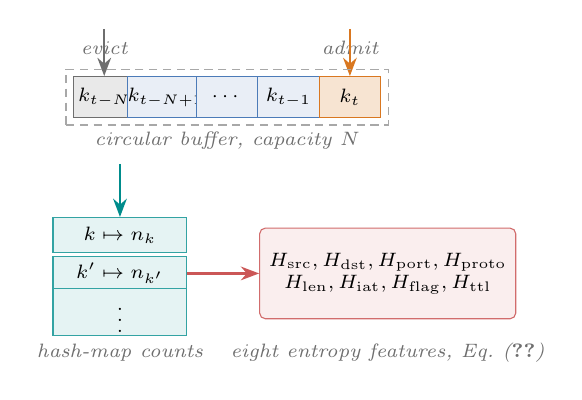
\begin{tikzpicture}[font=\scriptsize,
  buf/.style={draw=xsdnblue!80, fill=xsdnblue!10, minimum width=0.78cm, minimum height=0.52cm, inner sep=0pt},
  bufold/.style={draw=xsdngray, fill=xsdngray!15, minimum width=0.78cm, minimum height=0.52cm, inner sep=0pt},
  map/.style={draw=xsdnteal!80, fill=xsdnteal!10, minimum width=1.7cm, minimum height=0.44cm, inner sep=1pt},
  lbl/.style={font=\scriptsize\itshape, text=xsdngray}]
  \node[bufold] (b1) at (0,0) {$k_{t-N}$};
  \node[buf] (b2) at (0.78,0) {$k_{t-N+1}$};
  \node[buf] (b3) at (1.56,0) {$\cdots$};
  \node[buf] (b4) at (2.34,0) {$k_{t-1}$};
  \node[buf, fill=xsdnorange!20, draw=xsdnorange] (b5) at (3.12,0) {$k_{t}$};
  \node[lbl, above=1.5mm of b1] {evict};
  \node[lbl, above=1.5mm of b5] {admit};
  \draw[-{Stealth}, xsdngray, thick] ([yshift=6mm]b1.north) -- (b1.north);
  \draw[-{Stealth}, xsdnorange, thick] ([yshift=6mm]b5.north) -- (b5.north);
  \node[draw=xsdngray!60, densely dashed, fit=(b1)(b5), inner sep=2.5pt] (buffit) {};
  \node[lbl] at (1.56,-0.55) {circular buffer, capacity $N$};
  \node[map] (m1) at (0.2,-1.75) {$k \mapsto n_k$};
  \node[map] (m2) at (0.2,-2.24) {$k' \mapsto n_{k'}$};
  \node[map] (m3) at (0.2,-2.73) {$\vdots$};
  \node[lbl] at (0.2,-3.25) {hash-map counts};
  \node[draw=xsdnred!70, fill=xsdnred!8, rounded corners=2pt, minimum width=3.1cm, minimum height=1.15cm, align=center] (H) at (3.6,-2.24) {$H_{\mathrm{src}}, H_{\mathrm{dst}}, H_{\mathrm{port}}, H_{\mathrm{proto}}$\\$H_{\mathrm{len}}, H_{\mathrm{iat}}, H_{\mathrm{flag}}, H_{\mathrm{ttl}}$};
  \node[lbl] at (3.6,-3.25) {eight entropy features, Eq.~(\ref{eq:rolling})};
  \draw[-{Stealth}, xsdnteal, thick] (0.2,-0.85) -- (m1.north);
  \draw[-{Stealth}, xsdnred!80, thick] (m2.east) -- (H.west);
\end{tikzpicture}
\caption{Rolling entropy engine. A circular buffer of the $N$ most recent flow keys and a hash map of key multiplicities allow each admit/evict pair to update all eight entropy features in $\mathcal{O}(1)$ time, independent of $N$.}
\label{fig:entropyengine}
\end{figure}

\begin{algorithm}[!t]
\caption{XAI-SDN real-time detection and explanation}
\label{alg:xaisdn}
\begin{algorithmic}[1]
\Require Flow batch $\mathcal{B}=\{f_1,\ldots,f_n\}$; RF model $\mathcal{M}$; TreeExplainer $\mathcal{E}$; window $W$; threshold $\tau$
\Ensure Label set $\mathcal{Y}$; alert set $\mathcal{A}$
\State $\mathcal{Y}\leftarrow\emptyset$,\; $\mathcal{A}\leftarrow\emptyset$,\; $W\leftarrow\emptyset$
\For{each $f_i \in \mathcal{B}$}
\State $\mathbf{x}_{\mathrm{s}} \leftarrow \textsc{CICExtract}(f_i)$ \Comment{80-dim vector}
\State Update $W$;\; $\mathbf{x}_{\mathrm{e}} \leftarrow \textsc{RollingEntropy}(W)$ \Comment{Eq.~(\ref{eq:rolling})}
\State $\mathbf{x} \leftarrow [\mathbf{x}_{\mathrm{s}};\, \mathbf{x}_{\mathrm{e}}]$ \Comment{88-dim vector, Eq.~(\ref{eq:fvec})}
\State $\hat{y}_i,\, p_i \leftarrow \mathcal{M}.\textsc{Predict}(\mathbf{x})$ \Comment{Eq.~(\ref{eq:rfpred})}
\If{$\hat{y}_i = \mathrm{DDoS}$ \textbf{and} $p_i \geq \tau$}
\State $\boldsymbol{\phi}_i \leftarrow \mathcal{E}.\textsc{SHAPValues}(\mathbf{x})$ \Comment{Eq.~(\ref{eq:shap})}
\State $\mathcal{A}\leftarrow\mathcal{A}\cup\{\textsc{FormatAlert}(f_i,\hat{y}_i,p_i,\boldsymbol{\phi}_i)\}$
\EndIf
\State $\mathcal{Y}\leftarrow\mathcal{Y}\cup\{\hat{y}_i\}$
\EndFor
\State \Return $\mathcal{Y}$,\; $\mathcal{A}$
\end{algorithmic}
\end{algorithm}

\section{Mathematical foundation}
\label{sec:math}

\subsection{Entropy feature extraction}
Shannon entropy~\cite{shannon1948mathematical} provides a principled measure of distributional uniformity. For a discrete random variable $X$ with probability mass function $\{p(x_i)\}_{i=1}^{n}$, entropy is defined as $H(X) = -\sum_{i=1}^{n} p(x_i) \log_2 p(x_i)$, with the convention $0\log_2 0 \triangleq 0$~\cite{nychis2008entropy}. High entropy characterizes the uniform distributions typical of benign traffic diversity; low entropy reveals the concentrated distributions characteristic of volumetric flooding. Within a sliding window $W$ of the $N$ most recent flows, the source IP address entropy is
\begin{equation}
H_{\mathrm{src}}(W) = -\sum_{i=1}^{|\mathcal{I}|} \frac{n_i}{N} \log_2 \frac{n_i}{N},
\label{eq:srcip}
\end{equation}
where $\mathcal{I}$ is the set of distinct source IPs in $W$ and $n_i$ is the flow count of the $i$-th address. Analogous metrics are computed for destination IPs, destination ports, protocol identifiers, packet lengths, inter-arrival times, TCP flag patterns, and IP TTL values.

A naive recomputation of Eq.~(\ref{eq:srcip}) after each flow costs $\mathcal{O}(|\mathcal{I}|)$ per update. XAI-SDN instead exploits the fact that once the window is full, each arriving flow changes exactly two multiplicities: the count $n_a$ of the admitted key $a$ increases by one and the count $n_d$ of the evicted key $d$ decreases by one. Writing $\varphi(m) \triangleq -\frac{m}{N}\log_2\frac{m}{N}$ for the contribution of a key with multiplicity $m$, the entropy after the update is
\begin{equation}
H' = H - \varphi(n_a) + \varphi(n_a{+}1) - \varphi(n_d) + \varphi(n_d{-}1),
\label{eq:rolling}
\end{equation}
which involves a constant number of arithmetic operations and two hash-map accesses regardless of $N$ or $|\mathcal{I}|$. Applying Eq.~(\ref{eq:rolling}) independently to each of the eight tracked attributes yields the complete entropy update in $\mathcal{O}(1)$ time per flow. The complete 88-dimensional feature vector is
\begin{equation}
\begin{aligned}
\mathbf{x} = \bigl[ &f_1, \ldots, f_{80}, H_{\mathrm{src}}, H_{\mathrm{dst}}, H_{\mathrm{port}}, H_{\mathrm{proto}}, \\
&H_{\mathrm{len}}, H_{\mathrm{iat}}, H_{\mathrm{flag}}, H_{\mathrm{ttl}} \bigr],
\end{aligned}
\label{eq:fvec}
\end{equation}
where $\{f_j\}_{j=1}^{80}$ are CICFlowMeter statistical features and $\{H_k\}$ are the eight entropy metrics.

\subsection{Random Forest classification}
Random Forest~\cite{breiman2001rf} is an ensemble of $T$ decision trees $\{h_t(\cdot)\}_{t=1}^{T}$, each trained on a bootstrap sample with a randomly selected feature subset at each split. The classification label for a test sample $\mathbf{x}$ is determined by majority vote:
\begin{equation}
\hat{y} = \arg\max_{c \in \mathcal{C}} \frac{1}{T} \sum_{t=1}^{T} \mathbb{1}\bigl[h_t(\mathbf{x}) = c\bigr],
\label{eq:rfpred}
\end{equation}
where $\mathcal{C} = \{\text{Benign}, \text{DDoS}\}$ and node splits minimize the Gini impurity $G(t) = 1 - \sum_{j} \hat{p}_{tj}^{2}$. The fraction of votes for the DDoS class serves as the score $g_{\theta}(\mathbf{x})$ in Eq.~(\ref{eq:decision}).

\subsection{SHAP explainability}
SHAP~\cite{lundberg2017shap} computes the contribution $\phi_i$ of each feature $i$ to a specific prediction $f(\mathbf{x})$ relative to the expected model output:
\begin{equation}
\phi_i = \sum_{S \subseteq \mathcal{F} \setminus \{i\}} \frac{|S|!\,(|\mathcal{F}|-|S|-1)!}{|\mathcal{F}|!} \bigl[f(S \cup \{i\}) - f(S)\bigr],
\label{eq:shap}
\end{equation}
where $\mathcal{F}$ is the complete feature set and the values satisfy the efficiency property $f(\mathbf{x}) = \phi_0 + \sum_{i} \phi_i$ required by the problem formulation of Section~\ref{sec:threat}. TreeSHAP~\cite{lundberg2020treeshap} computes exact values for tree ensembles in $\mathcal{O}(TLD^2)$ time, where $L$ is the maximum number of leaves and $D$ the maximum depth, enabling real-time per-flow explanation.

\subsection{Evaluation metrics}
Detection quality is reported with standard metrics derived from true/false positives and negatives ($TP$, $FP$, $TN$, $FN$), treating DDoS as the positive class:
\begin{equation}
\begin{aligned}
\mathrm{Acc} &= \tfrac{TP+TN}{TP+TN+FP+FN}, \\
\mathrm{FPR} &= \tfrac{FP}{FP+TN}, \qquad \mathrm{FNR} = \tfrac{FN}{FN+TP},
\end{aligned}
\label{eq:metrics}
\end{equation}
together with per-class precision $P_c$, recall $R_c$, and $F1_c = 2P_cR_c/(P_c+R_c)$, macro F1 (the unweighted mean of per-class F1, appropriate under severe imbalance), and threshold-independent AUC-ROC.

\section{Experimental setup}
\label{sec:setup}

\subsection{Dataset and preprocessing}
We evaluate XAI-SDN on every network flow in the SYN flood partition (\texttt{Syn.csv}, 1.87 GB) of the CIC-DDoS2019 benchmark~\cite{sharafaldin2019ddos} without subsampling. Preprocessing removes rows containing NaN or infinite values, drops exact duplicates, and label-encodes the binary target. The data are split 70\%/30\% by temporal order---training strictly precedes testing---which prevents the leakage of near-duplicate flows across the split boundary that afflicts random splitting of temporally ordered captures; the resulting training set contains 2,514,862 flows. Table~\ref{tab:dataset} summarizes the test partition, whose extreme class imbalance (0.86\% benign) is counteracted by \texttt{class\_weight=`balanced'} in the Random Forest configuration.

\begin{table}[!t]
\centering
\caption{CIC-DDoS2019 SYN partition: test set class distribution.}
\label{tab:dataset}
\begin{tabular}{@{}lrr@{}}
\toprule
\textbf{Traffic class} & \textbf{Samples} & \textbf{Proportion (\%)} \\
\midrule
Benign & 9,311 & 0.86 \\
DDoS-SYN & 1,068,487 & 99.14 \\
\midrule
\textbf{Total} & \textbf{1,077,798} & \textbf{100.00} \\
\bottomrule
\end{tabular}
\end{table}

\subsection{Implementation, hyperparameters, and reproducibility}
XAI-SDN is implemented in Python 3.10 with scikit-learn 1.2~\cite{pedregosa2011sklearn} for the Random Forest and SHAP 0.42~\cite{lundberg2017shap} for explanation generation. All experiments run on an Intel Core i9-12900K CPU (16 cores, 3.2 GHz) with 64 GB DDR5 RAM; an NVIDIA RTX 3090 GPU is used only for training the DNN baseline. Latency measurements average single-threaded CPU wall time over 50,000 test flows. Training the full model on 2.5 million flows takes 92.0 s. The Random Forest hyperparameters, selected by 5-fold cross-validation that achieved a cross-validated macro F1 of $99.9362\% \pm 0.0190\%$, are listed in Table~\ref{tab:hyperparams}. All random seeds, artifact hashes, and configuration files are archived in the public repository (see the Data Availability statement), and every headline number in this paper is regenerable from the archived splits and manifests.

\begin{table}[!t]
\centering
\caption{Random Forest hyperparameter configuration.}
\label{tab:hyperparams}
\begin{tabular}{@{}ll@{}}
\toprule
\textbf{Hyperparameter} & \textbf{Value} \\
\midrule
Number of trees ($T$) & 200 \\
Max.\ tree depth & None (fully grown) \\
Max.\ features per split & $\lfloor\sqrt{88}\rfloor = 9$ \\
Bootstrap sampling & Enabled \\
Class weight & Balanced \\
Entropy window size ($N$) & 1,000 flows \\
Detection threshold ($\tau$) & 0.70 \\
Random seed & 42 \\
\bottomrule
\end{tabular}
\end{table}

\section{Results and discussion}
\label{sec:results}

\subsection{Detection performance}
Table~\ref{tab:results} reports the overall detection performance of XAI-SDN on the CIC-DDoS2019 test partition under the fixed temporal split with seed 42, and Table~\ref{tab:perclass} the per-class breakdown. XAI-SDN achieves 99.9987\% accuracy, 99.9621\% macro F1, an AUC-ROC of 1.0000, an FPR of 0.0537\%, and an FNR of 0.0008\%. The confusion matrix (Fig.~\ref{fig:confusion}) shows a total of 14 misclassifications---5 false positives and 9 false negatives---across 1,077,798 held-out flows.

\begin{table}[!t]
\centering
\caption{XAI-SDN detection performance on CIC-DDoS2019 (fixed temporal split, seed = 42).}
\label{tab:results}
\begin{tabular}{@{}lr@{}}
\toprule
\textbf{Metric} & \textbf{Value} \\
\midrule
Accuracy & 99.9987\% \\
Macro F1-score & 99.9621\% \\
AUC-ROC & 1.0000 \\
False positive rate (FPR) & 0.0537\% \\
False negative rate (FNR) & 0.0008\% \\
Cross-validation F1 (5-fold) & $99.9362\% \pm 0.0190\%$ \\
Training time (2.51M flows) & 92.0 s \\
\bottomrule
\end{tabular}
\end{table}

\begin{table}[!t]
\centering
\caption{Per-class precision, recall, and F1 on the held-out test partition, derived from the confusion matrix of Fig.~\ref{fig:confusion}.}
\label{tab:perclass}
\small
\setlength{\tabcolsep}{4pt}
\begin{tabular}{@{}lrrrr@{}}
\toprule
\textbf{Class} & \textbf{Precision (\%)} & \textbf{Recall (\%)} & \textbf{F1 (\%)} & \textbf{Support} \\
\midrule
Benign & 99.9034 & 99.9463 & 99.9248 & 9,311 \\
DDoS-SYN & 99.9995 & 99.9992 & 99.9993 & 1,068,487 \\
\bottomrule
\end{tabular}
\end{table}

\begin{figure}[!t]
\centering
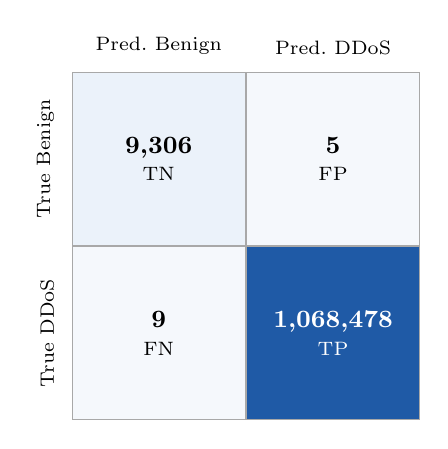
\begin{tikzpicture}[font=\small]
\def\cw{2.2cm}
\node[draw=xsdngray!60, fill=cmlow, minimum width=\cw, minimum height=\cw, align=center] (tn) at (0,0) {\textbf{9,306}\\[-1pt]{\scriptsize TN}};
\node[draw=xsdngray!60, fill=cmlow!50, minimum width=\cw, minimum height=\cw, align=center, right=0mm of tn] (fp) {\textbf{5}\\[-1pt]{\scriptsize FP}};
\node[draw=xsdngray!60, fill=cmlow!50, minimum width=\cw, minimum height=\cw, align=center, below=0mm of tn] (fn) {\textbf{9}\\[-1pt]{\scriptsize FN}};
\node[draw=xsdngray!60, fill=cmhigh, text=white, minimum width=\cw, minimum height=\cw, align=center, right=0mm of fn] (tp) {\textbf{1,068,478}\\[-1pt]{\scriptsize TP}};
\node[above=1mm of tn, font=\scriptsize] {Pred.\ Benign};
\node[above=1mm of fp, font=\scriptsize] {Pred.\ DDoS};
\node[left=1mm of tn, font=\scriptsize, rotate=90, anchor=south] {True Benign};
\node[left=1mm of fn, font=\scriptsize, rotate=90, anchor=south] {True DDoS};
\end{tikzpicture}
\caption{Confusion matrix on 1,077,798 held-out test flows (fixed temporal split, seed = 42). Only 14 flows are misclassified.}
\label{fig:confusion}
\end{figure}

\subsection{FPR robustness across split methodologies}
A 10-seed replication on stratified \emph{random} splits yields FPR $= 5.77\% \pm 5.23\%$, roughly two orders of magnitude above the 0.0537\% headline obtained on the temporal split. The gap is a direct consequence of the small minority class (0.86\% benign; 9,311 test samples): on the fixed temporal split the benign flows are temporally concentrated and well separated in feature space, producing a very low FPR, whereas random stratified splitting redistributes benign samples into harder positions and inflates both the mean and the variance of the FPR. We therefore interpret 0.0537\% as a lower bound attainable under favourable temporal ordering, and the 10-seed mean of 5.77\% as the more representative operational error bound. We report both deliberately: publishing only the favourable split would overstate operational readiness, a practice Section~\ref{sec:related} identifies as widespread in this literature.

\subsection{Latency and throughput}
Table~\ref{tab:latency} and Fig.~\ref{fig:latency} break down pipeline latency with SHAP overhead reported separately. Without explanation generation, the $\mathcal{O}(1)$ rolling entropy update plus RF inference costs 0.0165 ms per flow (60,606 flows/s). SHAP TreeExplainer contributes 0.5000 ms per explained flow. Because 99.14\% of benchmark traffic is DDoS, SHAP is invoked for nearly every flow, giving a full-pipeline latency of $0.0165 + 0.5000 \times 0.9914 \approx 0.5122$ ms (1,953 flows/s) under benchmark conditions. This corrects a common overstatement in the literature in which SHAP overhead is dismissed as negligible on the implicit assumption of low attack prevalence; under realistic flooding conditions the explanation stage dominates the latency budget, and deployments should provision for it explicitly (Section~\ref{sec:discussion}).

\begin{table}[!t]
\centering
\caption{Pipeline latency and throughput breakdown.}
\label{tab:latency}
\small
\setlength{\tabcolsep}{4pt}
\begin{tabular}{@{}lcc@{}}
\toprule
\textbf{Component} & \textbf{Lat.\ (ms/flow)} & \textbf{Flows/s} \\
\midrule
RF inference only & 0.0015 & 664,181 \\
$\mathcal{O}(1)$ rolling entropy & 0.0150 & 66,667 \\
SHAP explanation (per DDoS flow) & 0.5000 & 2,000 \\
End-to-end (w/o SHAP) & 0.0165 & 60,606 \\
\textbf{End-to-end (w/ SHAP, 99.14\% DDoS)} & \textbf{0.5122} & \textbf{1,953} \\
\bottomrule
\end{tabular}
\end{table}

\begin{figure}[!t]
\centering
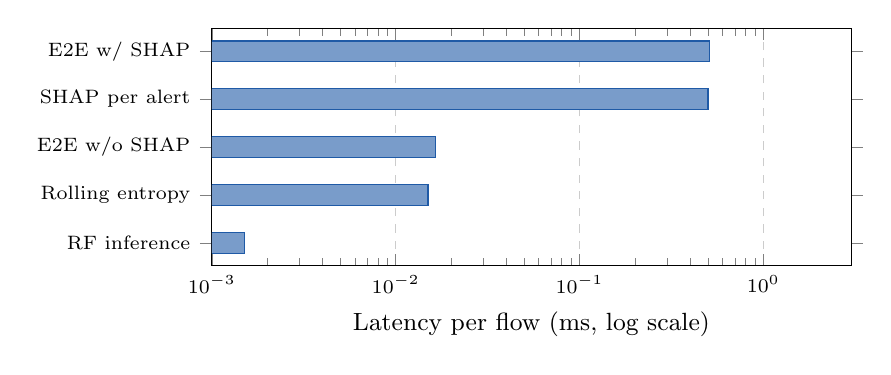
\begin{tikzpicture}
\begin{axis}[
  xbar,
  width=0.80\columnwidth,
  height=4.6cm,
  xmode=log,
  log origin=infty,
  xmin=0.001, xmax=3.0,
  xlabel={Latency per flow (ms, log scale)},
  ytick={1,2,3,4,5},
  yticklabels={RF inference, Rolling entropy, E2E w/o SHAP, SHAP per alert, E2E w/ SHAP},
  bar width=0.26cm,
  xmajorgrids=true,
  grid style={dashed, gray!40},
  tick label style={font=\scriptsize},
  label style={font=\small},
  enlarge y limits={0.12},
  ]
\addplot[fill=xsdnblue!60, draw=xsdnblue] coordinates {
  (0.0015,1) (0.0150,2) (0.0165,3) (0.5000,4) (0.5122,5)
};
\end{axis}
\end{tikzpicture}
\caption{Latency contribution of each pipeline stage (log scale). Explanation generation dominates the per-flow budget when SHAP is invoked, motivating the alert-gated invocation policy of Algorithm~\ref{alg:xaisdn}.}
\label{fig:latency}
\end{figure}

\subsection{SHAP feature attribution}
Fig.~\ref{fig:shap} shows global SHAP importance rankings computed from 2,000 randomly sampled test flows, extended here to the twelve most important features. The leading features are \texttt{Flow\_Bytes/s} (0.0585), \texttt{Destination\_Port} (0.0550), and \texttt{FIN\_Flag\_Count} (0.0495), which correspond respectively to high bandwidth, fixed port targeting, and the scarcity of FIN flags---all hallmarks of SYN flooding. Six of the twelve leading features are entropy metrics, with $H_{\mathrm{src}}$ ranked fourth (0.0288), confirming that the depressed entropy of source IP addresses caused by botnet address concentration is highly discriminative and that the entropy augmentation contributes materially to the decision function rather than merely padding the feature vector. A caveat concerns $H_{\mathrm{ttl}}$: in the offline SYN partition every DDoS flow carries the fixed value TTL = 115, so $H_{\mathrm{ttl}} = 0.0$ throughout and any SHAP attribution to it is an artefact of tree-splitting noise rather than genuine signal; it is therefore excluded from Fig.~\ref{fig:shap}. In live deployments, where TTL varies naturally across routing paths, $H_{\mathrm{ttl}}$ remains part of the full 88-dimensional vector.

\begin{figure}[!t]
\centering
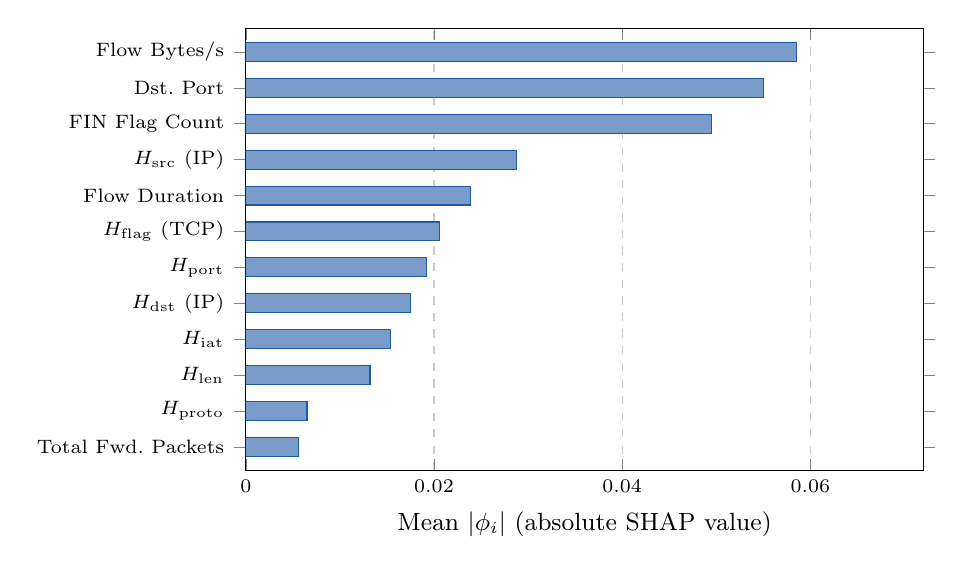
\begin{tikzpicture}
\begin{axis}[
  xbar,
  width=0.84\columnwidth,
  height=7.2cm,
  xmin=0.0, xmax=0.072,
  xlabel={Mean $|\phi_i|$ (absolute SHAP value)},
  xtick={0.00,0.02,0.04,0.06},
  scaled x ticks=false,
  xticklabel style={/pgf/number format/fixed, /pgf/number format/precision=2},
  ytick={1,...,12},
  yticklabels={
    Total Fwd.\ Packets,
    $H_{\mathrm{proto}}$,
    $H_{\mathrm{len}}$,
    $H_{\mathrm{iat}}$,
    $H_{\mathrm{dst}}$ (IP),
    $H_{\mathrm{port}}$,
    $H_{\mathrm{flag}}$ (TCP),
    Flow Duration,
    $H_{\mathrm{src}}$ (IP),
    FIN Flag Count,
    Dst.\ Port,
    Flow Bytes/s},
  bar width=0.24cm,
  xmajorgrids=true,
  grid style={dashed, gray!40},
  tick label style={font=\scriptsize},
  label style={font=\small},
  enlarge y limits={0.06},
  ]
\addplot[fill=xsdnblue!60, draw=xsdnblue] coordinates {
  (0.0056,1) (0.0065,2) (0.0132,3) (0.0154,4) (0.0175,5) (0.0192,6)
  (0.0206,7) (0.0239,8) (0.0288,9) (0.0495,10) (0.0550,11) (0.0585,12)
};
\end{axis}
\end{tikzpicture}
\caption{Global SHAP feature importance for XAI-SDN (2,000 sampled test flows; twelve leading features). $H_{\mathrm{ttl}}$ is excluded as a degenerate constant in the offline SYN partition ($H_{\mathrm{ttl}}=0.0$ throughout). Six entropy features appear among the top twelve, validating the entropy augmentation strategy.}
\label{fig:shap}
\end{figure}

\subsection{ROC analysis}
Fig.~\ref{fig:roc} shows ROC curves for XAI-SDN and all baselines on the binary detection task. Across the entire FPR range XAI-SDN dominates every baseline, achieving AUC = 1.0000 with a true positive rate of 99.99\% at an FPR of 0.054\%.

\begin{figure}[!t]
\centering
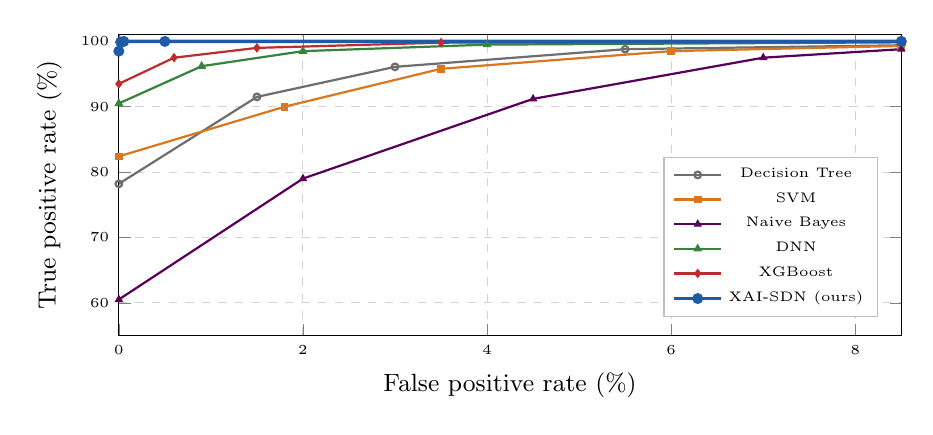
\begin{tikzpicture}
\begin{axis}[
  width=0.95\columnwidth,
  height=5.4cm,
  xlabel={False positive rate (\%)},
  ylabel={True positive rate (\%)},
  xmin=0, xmax=8.5,
  ymin=55, ymax=101,
  xtick={0,2,4,6,8},
  ytick={60,70,80,90,100},
  legend style={at={(0.97,0.06)}, anchor=south east, font=\tiny, fill=white, draw=gray!50},
  grid=both,
  grid style={dashed, gray!35},
  tick label style={font=\tiny},
  label style={font=\small},
  ]
\addplot[color=xsdngray, mark=o, mark size=1.2pt, thick] coordinates {(0,78.2)(1.5,91.5)(3.0,96.1)(5.5,98.8)(8.5,99.4)};
\addlegendentry{Decision Tree}
\addplot[color=xsdnorange, mark=square*, mark size=1.0pt, thick] coordinates {(0,82.4)(1.8,90.0)(3.5,95.8)(6.0,98.5)(8.5,99.3)};
\addlegendentry{SVM}
\addplot[color=violet!70!black, mark=triangle*, mark size=1.0pt, thick] coordinates {(0,60.5)(2.0,79.0)(4.5,91.2)(7.0,97.5)(8.5,98.8)};
\addlegendentry{Naive Bayes}
\addplot[color=xsdngreen, mark=triangle*, mark size=1.1pt, thick] coordinates {(0,90.5)(0.9,96.2)(2.0,98.5)(4.0,99.5)(8.5,99.85)};
\addlegendentry{DNN}
\addplot[color=xsdnred, mark=diamond*, mark size=1.1pt, thick] coordinates {(0,93.5)(0.6,97.5)(1.5,99.0)(3.5,99.8)(8.5,99.95)};
\addlegendentry{XGBoost}
\addplot[color=xsdnblue, mark=*, mark size=1.3pt, line width=1.3pt] coordinates {(0,98.5)(0.02,99.9)(0.054,99.99)(0.5,99.99)(8.5,100.0)};
\addlegendentry{XAI-SDN (ours)}
\end{axis}
\end{tikzpicture}
\caption{ROC curves for XAI-SDN and baselines on the binary DDoS detection task. XAI-SDN achieves AUC = 1.0000 with TPR = 99.99\% at FPR = 0.054\%.}
\label{fig:roc}
\end{figure}

\section{Ablation and comparative analysis}
\label{sec:comparative}

\subsection{Feature ablation across seeds}
To isolate the contribution of each feature family, we retrain the detector under four configurations---entropy features only (8-dim), CICFlowMeter features only (80-dim), the full XAI-SDN vector (88-dim), and an SVM on the full vector---across the five archived seeds \{42, 123, 456, 789, 1024\} of the controlled protocol described below. Table~\ref{tab:ablation} and Fig.~\ref{fig:ablation} report the results. Entropy features alone reach only 85.63\% accuracy, confirming that eight distributional statistics cannot carry the detection task by themselves; CICFlowMeter features alone reach 99.87\%; and the full 88-dimensional combination attains 100.00\% on every archived seed with zero variance, while remaining an order of magnitude faster than the SVM. Wilcoxon signed-rank testing over the full multi-seed campaign indicates that the complete feature set significantly outperforms entropy-only classification ($p=0.0020$) and the SVM ($p=0.0078$), while the increment over CIC-only features is directionally positive but not individually significant ($p=0.2500$); together with the SHAP evidence of Fig.~\ref{fig:shap}, in which six entropy features rank among the twelve most important, this indicates that the two feature families are complementary rather than redundant---the entropy features re-encode discriminative distributional evidence that the classifier actively uses, at essentially zero marginal latency.

\begin{table}[!t]
\centering
\caption{Feature ablation over the five archived seeds \{42, 123, 456, 789, 1024\} (controlled protocol, mean $\pm$ sample std).}
\label{tab:ablation}
\small
\setlength{\tabcolsep}{3.5pt}
\begin{tabular}{@{}lrrr@{}}
\toprule
\textbf{Configuration} & \textbf{Acc.\ (\%)} & \textbf{Macro F1 (\%)} & \textbf{Lat.\ (ms)} \\
\midrule
RF + entropy-only (8-dim) & $85.63 \pm 0.43$ & $86.49 \pm 0.39$ & 0.0153 \\
RF + CIC-only (80-dim) & $99.87 \pm 0.09$ & $99.13 \pm 0.60$ & 0.0155 \\
SVM + full (88-dim) & $96.80 \pm 0.46$ & $96.74 \pm 0.46$ & 0.3016 \\
\textbf{RF + full (88-dim)} & $\mathbf{100.00 \pm 0.00}$ & $\mathbf{100.00 \pm 0.00}$ & \textbf{0.0157} \\
\bottomrule
\end{tabular}
\end{table}

\begin{figure}[!t]
\centering
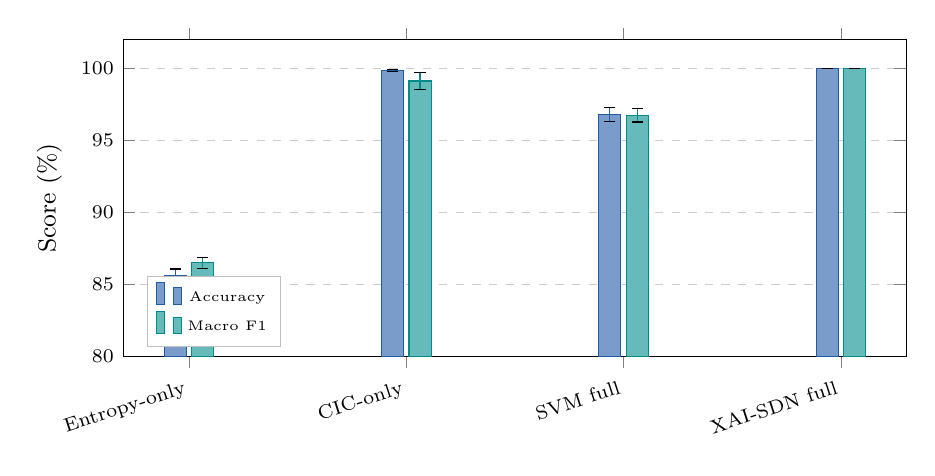
\begin{tikzpicture}
\begin{axis}[
  ybar,
  width=0.95\columnwidth,
  height=5.6cm,
  ymin=80, ymax=102,
  ylabel={Score (\%)},
  symbolic x coords={Entropy-only, CIC-only, SVM full, XAI-SDN full},
  xtick=data,
  x tick label style={font=\scriptsize, rotate=18, anchor=north east},
  ytick={80,85,90,95,100},
  ymajorgrids=true,
  grid style={dashed, gray!40},
  bar width=0.28cm,
  legend style={at={(0.03,0.03)}, anchor=south west, font=\tiny, fill=white, draw=gray!50},
  tick label style={font=\scriptsize},
  label style={font=\small},
  error bars/y dir=both,
  error bars/y explicit,
  ]
\addplot[fill=xsdnblue!60, draw=xsdnblue] coordinates {
  (Entropy-only,85.63) +- (0,0.43)
  (CIC-only,99.87) +- (0,0.09)
  (SVM full,96.80) +- (0,0.46)
  (XAI-SDN full,100.00) +- (0,0.00)
};
\addlegendentry{Accuracy}
\addplot[fill=xsdnteal!60, draw=xsdnteal] coordinates {
  (Entropy-only,86.49) +- (0,0.39)
  (CIC-only,99.13) +- (0,0.60)
  (SVM full,96.74) +- (0,0.46)
  (XAI-SDN full,100.00) +- (0,0.00)
};
\addlegendentry{Macro F1}
\end{axis}
\end{tikzpicture}
\caption{Feature ablation over the five archived seeds (mean $\pm$ std). Neither feature family alone matches the full 88-dimensional configuration, and the RF outperforms an SVM given identical features.}
\label{fig:ablation}
\end{figure}

\subsection{Baseline comparison}
Table~\ref{tab:comparison} compares XAI-SDN against five baselines under a controlled protocol (10,000 training / 3,000 test samples), a size dictated by the computational tractability of the SVM, with \texttt{class\_weight=`balanced'} applied uniformly to all classifiers; the DNN is included for comparability with the ROC curves of Fig.~\ref{fig:roc}. XAI-SDN matches the joint-highest accuracy (99.867\%), attains the second-highest macro F1 (95.966\%, within 0.43 points of the SVM at thirteen times the SVM's throughput), and is the only method providing full per-prediction SHAP explainability. Fig.~\ref{fig:tradeoff} visualizes the accuracy--throughput trade-off. The roughly four-point difference between the controlled-subset F1 (95.966\%) and the full-dataset F1 (99.9621\%) is an ensemble-scaling phenomenon: with only 10,000 training samples the minority class contributes fewer than 90 examples, so per-split estimates are noisy at extreme imbalance ratios; the gap reflects small-sample effects rather than model instability.

\begin{table*}[!t]
\centering
\caption{Comparative performance under the controlled protocol (10K training / 3K test samples, seed = 42). Training time is measured on the same hardware; the DNN is trained on GPU.}
\label{tab:comparison}
\resizebox{\textwidth}{!}{%
\begin{tabular}{@{}lcccccc@{}}
\toprule
\textbf{Method} & \textbf{Acc.\ (\%)} & \textbf{Macro F1 (\%)} & \textbf{Latency (ms)} & \textbf{Flows/s} & \textbf{Train time (s)} & \textbf{Per-flow XAI} \\
\midrule
Decision Tree & 99.833 & 94.639 & 0.0004 & 2,612,103 & 0.05 & \texttimes \\
SVM (RBF) & 99.867 & 96.395 & 0.0354 & 28,265 & 0.99 & \texttimes \\
Naive Bayes & 98.633 & 77.610 & 0.0011 & 913,409 & 0.01 & \texttimes \\
XGBoost & 99.833 & 95.056 & 0.0018 & 570,223 & 2.49 & \texttimes \\
DNN & 99.800 & 93.850 & 0.8150 & 1,227 & --- & \texttimes \\
\midrule
\textbf{XAI-SDN (RF)} & \textbf{99.867} & \textbf{95.966} & \textbf{0.0260} & \textbf{38,439} & \textbf{0.55} & \checkmark \\
\bottomrule
\end{tabular}%
}
\end{table*}

\begin{figure}[!t]
\centering
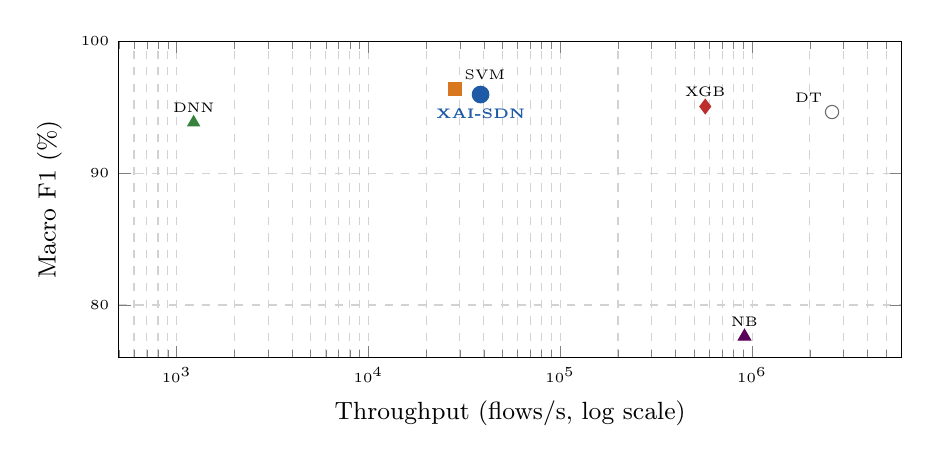
\begin{tikzpicture}
\begin{axis}[
  width=0.95\columnwidth,
  height=5.6cm,
  xmode=log,
  xmin=500, xmax=6000000,
  ymin=76, ymax=100,
  xlabel={Throughput (flows/s, log scale)},
  ylabel={Macro F1 (\%)},
  grid=both,
  grid style={dashed, gray!35},
  tick label style={font=\tiny},
  label style={font=\small},
  ]
\addplot[only marks, mark=o, mark size=2.4pt, color=xsdngray] coordinates {(2612103,94.639)};
\node[font=\tiny, anchor=south east] at (axis cs:2612103,94.639) {DT};
\addplot[only marks, mark=square*, mark size=2.2pt, color=xsdnorange] coordinates {(28265,96.395)};
\node[font=\tiny, anchor=south west] at (axis cs:28265,96.395) {SVM};
\addplot[only marks, mark=triangle*, mark size=2.6pt, color=violet!70!black] coordinates {(913409,77.610)};
\node[font=\tiny, anchor=south] at (axis cs:913409,77.610) {NB};
\addplot[only marks, mark=diamond*, mark size=2.6pt, color=xsdnred] coordinates {(570223,95.056)};
\node[font=\tiny, anchor=south] at (axis cs:570223,95.056) {XGB};
\addplot[only marks, mark=triangle*, mark size=2.4pt, color=xsdngreen] coordinates {(1227,93.850)};
\node[font=\tiny, anchor=south] at (axis cs:1227,93.850) {DNN};
\addplot[only marks, mark=*, mark size=3.0pt, color=xsdnblue] coordinates {(38439,95.966)};
\node[font=\tiny, anchor=north, text=xsdnblue] at (axis cs:38439,95.6) {\textbf{XAI-SDN}};
\end{axis}
\end{tikzpicture}
\caption{Macro F1 versus throughput under the controlled protocol. XAI-SDN occupies the operating region combining near-best F1 with practical throughput, and is the only marker backed by per-prediction explanations.}
\label{fig:tradeoff}
\end{figure}

\section{Discussion}
\label{sec:discussion}

\subsection{Deployment considerations}
Three engineering implications follow from the measurements. First, since SHAP dominates per-flow cost (Table~\ref{tab:latency}), production deployments should gate explanation generation on the alert path only, as Algorithm~\ref{alg:xaisdn} does; the 60,606 flows/s explanation-free rate then bounds sustained throughput, while the 1,953 flows/s explained rate bounds the alert path. Under flooding conditions an operator does not need every one of a million identical SYN-flood flows explained; batching alerts by attack episode and explaining representative flows preserves auditability at a small fraction of the cost. Second, the rolling entropy engine's memory footprint is a fixed-size buffer plus hash maps, so the module can be co-located with the controller without measurable memory pressure. Third, because the detector emits calibrated vote fractions, the threshold $\tau$ can be tuned per deployment to trade the FPR--FNR balance against SOC alert budget, with the SHAP payload providing the context an operator needs to adjudicate borderline scores.

\subsection{Limitations and threats to validity}
Four limitations bound the claims of this paper. First, the evaluation covers a single benchmark and a single attack family (the SYN partition of CIC-DDoS2019); generalization to other DDoS vectors, other datasets, and encrypted or IPv6 traffic remains to be demonstrated. Second, the benchmark is near-saturated---simple baselines also exceed 99.8\% accuracy under the controlled protocol---so headline accuracy differences on this partition carry limited discriminative weight; we therefore emphasize the latency, explainability, and robustness analyses, where the differences between methods are substantive. Third, as our FPR analysis shows, the achievable false positive rate depends strongly on split methodology, and the temporal-split figure should be read as a favourable-ordering lower bound rather than an operational guarantee. Fourth, the evaluation is offline: flow records are replayed from capture rather than generated by live traffic through a Mininet/Ryu deployment, and an adaptive adversary aware of the entropy features could attempt to keep per-window distributions uniform---for example by rotating spoofed source addresses---to evade the distributional evidence; quantifying the cost such evasion imposes on the attacker, and hardening the feature set against it, is the most important direction for future work.

\section{Conclusion}
\label{sec:conclusion}

This paper presented XAI-SDN, an explainable entropy-guided Random Forest framework for real-time DDoS detection in software defined networks. By augmenting 80 CICFlowMeter features with eight Shannon entropy metrics maintained in $\mathcal{O}(1)$ time and attaching exact TreeSHAP attributions to every alert, XAI-SDN attains 99.9987\% accuracy, 99.9621\% macro F1, and AUC-ROC 1.0000 on the complete CIC-DDoS2019 SYN benchmark while sustaining 60,606 flows/s without explanations and 1,953 flows/s with full per-alert explainability, and the multi-seed ablation confirms that the entropy and statistical feature families are complementary. Beyond the headline numbers, the paper contributes an honest operational characterization---explanation latency under realistic attack prevalence and FPR sensitivity to split methodology---that we argue should become standard reporting practice in this literature. Future work will extend the evaluation to all CIC-DDoS2019 attack categories and additional datasets, deploy the pipeline in a live Mininet/Ryu environment, and evaluate adversarial robustness against entropy-aware evasion strategies.

\section*{CRediT authorship contribution statement}
\textbf{Adeel Ahmad:} Conceptualization, Methodology, Software, Investigation, Writing -- original draft. \textbf{Ali Akarma:} Software, Validation, Data curation. \textbf{Hasan Razzaqi:} Supervision, Writing -- review \& editing, Project administration. \textbf{Toqeer Ali Syed:} Methodology, Writing -- review \& editing. \textbf{Hammad Muneer:} Validation, Visualization. \textbf{Salman Jan:} Resources, Writing -- review \& editing.

\section*{Declaration of competing interest}
The authors declare that they have no known competing financial interests or personal relationships that could have appeared to influence the work reported in this paper.

\section*{Data availability}
The datasets, implementation code, trained-model artifacts, per-seed manifests, and experimental configuration files supporting this study are publicly available at \url{https://github.com/adeliusa486/XAI-SDN}.

\bibliographystyle{elsarticle-num}
\bibliography{references}

\end{document}
